\documentclass{standalone}
\usepackage[T1]{fontenc}
\renewcommand*\familydefault{\sfdefault} %%
\usepackage{sfmath}
\usepackage{pgfplots}

\begin{document}


\tikzset{every picture/.style={line width=0.75pt}} %set default line width to 0.75pt        

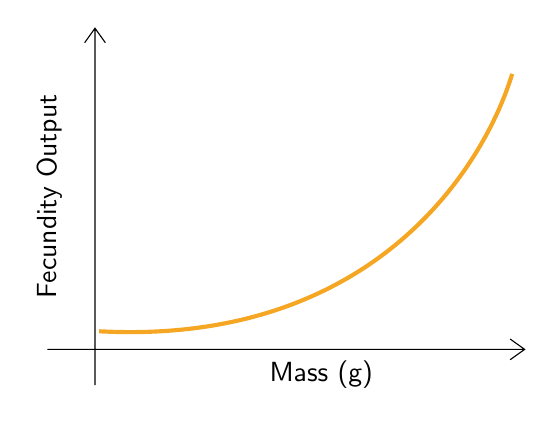
\begin{tikzpicture}[x=0.75pt,y=0.75pt,yscale=-1,xscale=1]
%uncomment if require: \path (0,300); %set diagram left start at 0, and has height of 300

%Shape: Axis 2D [id:dp3114220934792187] 
\draw  (24,200.73) -- (254,200.73)(47,46) -- (47,217.92) (247,195.73) -- (254,200.73) -- (247,205.73) (42,53) -- (47,46) -- (52,53)  ;
%Curve Lines [id:da1333162265444947] 
\draw [color={rgb, 255:red, 245; green, 166; blue, 35 }  ,draw opacity=1 ][line width=1.5]    (49,192) .. controls (180,199) and (234,114) .. (248,68) ;



% Text Node
\draw (156,213) node  [align=left] {Mass (g)};
% Text Node
\draw (25,127) node [rotate=-270.08] [align=left] {Fecundity Output};


\end{tikzpicture}
\end{document}